This section describes the various systematic uncertainties considered in this analysis. 
There are systematic uncertainties on both the jet and calorimeter clusters that are used in this measurements.
Both the jet and calorimeter cluster systematic uncertainties can be broadly classified into three categories: calibration, selection efficiency and unfolding uncertainties.
The calibration and selection efficiency uncertainties are studied for the jet and calorimeter clusters independently and then propagated through the full unfolding procedure while the unfolding uncertainties are studied for the combined jet and calorimeter cluster response. Note, we take a conservative treatment of the jet and calorimeter cluster calibration and selection efficiency uncertainties by studying their effects as uncorrelated. We believe this is a reasonable method for this analysis since the largest uncertainty contributions are from the hadronic response and noise effects on the calorimeter clusters. The noise effects should be negligible for the jets used in this analysis while the hadronic response uncertainty used for the calorimeter clusters is no longer being used for the scale uncertainty on the jets, instead a more precise in-situ photon-jet calibration study is used. 

The full set of systematic uncertainties with details on their evaluation in the analysis chain are listed in Table \ref{table:full_systematics}. Further details on the determination of each systematic uncertainty is given in the following sections. \newline
\begin{table}[ht]
\centering
\begin{tabular}{|c|c|c|c|}
\hline
Systematic Uncertainty & Type & Data/Sim Varied \\ \hline
JES Uncertainty & Calibration & Simulation \\ \hline
JER Uncertainty & Calibration & Simulation \\ \hline
Jet trigger efficiency & Selection efficiency & Data \\ \hline
Calorimeter tower calibration & Calibration & Data \\ \hline
Calorimeter tower resolution & Calibration & Simulation \\ \hline
Calorimeter hadronic response & Calibration & Data \\ \hline
Topocluster noise threshold & Selection efficiency & Data \& Sim \\ \hline
Pileup correction & Selection efficiency & Data \\ \hline
MBD vertex efficiency & Selection efficiency & Data \\ \hline
Prior reweighting & Unfolding & Simulation \\ \hline
Herwig response & Unfolding & Simulation \\ \hline
\end{tabular}
\caption{Full set of systematic uncertainties.}
\end{table}
\label{table:full_systematics}

\subsection{Jet Systematic Uncertainties}

\subsubsection{JES Uncertainty}
The same JES uncertainty used in PPG08 and PPG09 \cite{ppg08AN,ppg09AN} is applied to this analysis. 
This uncertainty is being finalized but is currently derived from the scale difference between data and MC in the in-situ photon-jet calibration studies and results in a 2.5\% uncertainty on the jet energy scale. 
The JES up and down uncertainties are applied to the simulation JES term and propagated through the unfolding procedure as a variation on the simulation response matrix.
More information on the JES can be found in the PPG09 analysis note~\cite{ppg09AN} and the JES uncertainty can be found in the photon-jet in situ jet energy calibration analysis note \cite{in_situ_note}.

\subsubsection{JER Uncertainty}
The same JER uncertianty used in PPG08 and PPG09 \cite{ppg08AN,ppg09AN} is applied to this analysis. 
This uncertiantiy is derived from the differences in JER results extracted from two different data-driven methods, the dijet balance method and the bisector method and results in a 1.8\% uncertainty on the jet energy resolution.
The JER up and down uncertainties are applied to the simulation JER smearing term and propagated through the unfolding procedure as a variation on the simulation response matrix.
More information on the data driven JER uncertainty studies preformed by PPG08 can be found in the PPG08 analysis note \cite{ppg08AN}.

\subsubsection{Jet trigger efficiency}
The jet trigger efficinecy is derived by varying the jet fit parameters of the jet trigger efficiency fit function by to find the 1$\sigma$ variations in the jet trigger efficiency.
The jet trigger efficiency is then propagated through the unfolding procedure through a variation data histogram to find the systematic uncertainty on the UE measurement.

\subsection{Calorimeter Cluster Systematic Uncertainties}

\subsubsection{Calorimeter tower calibration}
The absolute energy scale calibration uncertainties of the calorimeter towers for both the EMCal and HCals are determined from the uncertainties in the calorimeter calibration methodology and are described in more detail in \cite{ppg03AN,Seidlitz1}.
A systematic uncertainty on the overall scale of the EMCal absolute calibration of 0.5\% uncertainty based on the range in calibration values from \href{https://indico.bnl.gov/login/?next=/event/31859/contributions/120756/attachments/68548/117758/EMCal_toyMC_calib_20260302.pdf}{toy MC studies of the mass and width of the $\pi^{0}$ and $\eta$ peaks} is applied to the EMCal towers included in the topoclusters.
A systematic uncertainty on the overall scale of the OHCal absolute calibration of 1\% uncertainty based on the residual run dependence of the OHCal calibration in Run 2024 is applied to the OHCal towers included in the topoclusters.
A systematic uncertainty on the overall scale of the IHCal absolute calibration of 10\% uncertainty based on the Data/MC differences in the \detdeta extracted from the IHCal in \cite{ppg03AN} is applied to the IHCal towers included in the topoclusters.
An additional $\eta$ dependent scale uncertainty ranging from $-10\%$ to $10\%$ is applied to the OHCal towers included in the topoclusters based on the Data/MC differences in the \detdeta extracted from the OHCal in \cite{ppg03AN}.
The $\eta$ dependent scale uncertainty values as a function of OHCal $i\eta$ bin used for this analysis are extracted from the MC/Data curve for AMPT are shown in Figure~\ref{fig:ohcal_eta_dep_scale_uncertainty}.
\begin{figure}
    \centering
    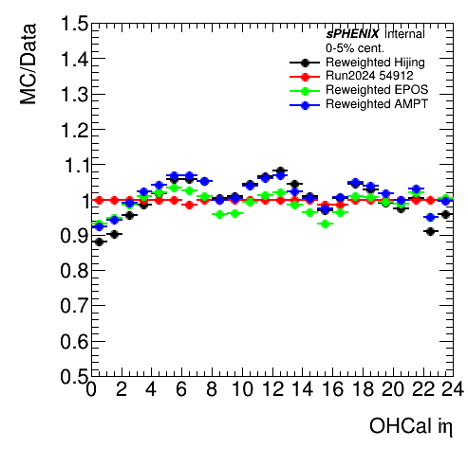
\includegraphics[width=0.7\linewidth]{Figures/systematics/eta_dependent_scale_uncertainty.png}
    \caption{Additional $\eta$ dependent scale uncertainty values as a function of OHCal $i\eta$ bin based on the Data/MC differences in the \detdeta extracted from the OHCal in \cite{ppg03AN}. Blue curve showing the MC/Data differences using AMPT is used for this scale uncertainty.}
    \label{fig:ohcal_eta_dep_scale_uncertainty}
\end{figure}
For all of these calorimeter tower calibration uncertainties, the overall scale of individual calorimeter towers included in the topoclusters is varied by the corresponding calibration uncertainty and this variation is propagated through the unfolding procedure as a variation on the data histogram.
The overall effect of these calorimeter tower calibration uncertainties on the UE measurement is found to be at the 1\% level for all leading jet $p_T$ bins.

\subsubsection{Calorimter tower resolution}
The calorimeter tower resolution uncertainty is derived from the Data/MC differences seen in the EMCal clusters in the \href{https://indico.bnl.gov/login/?next=/event/31859/contributions/120756/attachments/68548/117758/EMCal_toyMC_calib_20260302.pdf}{toy MC studies of the mass and width of the $\pi^{0}$ and $\eta$ peaks} calorimeter calibrations group and neutral mesons PPG11 and data-driven JER studies in PPG08 \cite{ppg08AN}.
Two difference resolution variations are applied to the topoclusters used for the UE measurement: a variation on the position resolution of the topoclusters and a variation on the energy resolution of the topoclusters.

The position resolution of the topoclusters is varied by 0.005 radian which was found to be the difference in position resolution factors between different toy MC models that were used to accurately fit both the mass and width of the $\pi^{0}$ and $\eta$ peaks in data and MC in the EMCal cluster calibration studies.
The variation in the position resolution of the topoclusters should have a negligible effect on the UE measurement as the UE measurement is summed over a large region of 2.2 units in $\eta$ and $2 \pi/ 3$ radians in $\phi$.
However, this variation is tested to check for any effects from inflow and outflow of topoclusters in and out of the transverse region due to the position resolution of the topoclusters.
This uncertainty is applied by varying the position of the topoclusters in simulation by 0.005 radians and propagating this uncertainty through the unfolding procedure as a variation on the data histogram.
The overall effect of this position resolution variation on the UE measurement is found to be negligible ($<$ 0.1\%).

Two resolution studies are then used to constrain the calorimeter topocluster energy resolution uncertainty.
For both lower energy EMCal clusters and higher energy full calorimeter jets, the Data/MC differences in the resolution are found to be around 8-10\% with studies of the JER showing the majority of the Data/MC differences in resolution come from the EMCal contributions.
Therefore, the topocluster energy resolution differences between data and MC are constrained by these two different studies of the calorimeter resolution and a 8\% smearing on the topocluster energies is applied in simulation and propagated through the unfolding procedure as a variation on the simulation response matrix to find the cluster energy resolution systematic uncertainty on the UE measurement.
The total effect of this energy resolution variation on the on the UE measurement is found to be at the 1\% level for all leading jet $p_T$ bins.

\subsubsection{Calorimeter hadronic response}
The uncertainty in the calorimeter hadronic energy scale is derived from Data/MC differences seen in the EMCal and HCal test beam paper~\cite{emcal_beamtest,emcal_hcal_beamtest}.
The uncertainty is applied by varying the overall scale of the topoclusters by 4.9\% and propagating this uncertainty through the unfolding procedure as a variation on the data histogram.
This uncertainty is the same as the hadronic response uncertainty applied to the \detdeta analysis in PPG03 \cite{ppg03AN}.

\subsubsection{Topocluster noise threshold}
The topocluster noise threshold are varied between the 2 and 3 sigma thresholds studied in the topocluster noise study in Section~\ref{sec:towerreco} to test the impact of noise on the topocluster reconstruction and extracted calorimeter cluster total energy.
This uncertainty is applied by varying the topocluster noise threshold in both simulation and data and is propagated through the unfolding procedure with variations on both the data histogram and the simulation response matrix.
The overall effect of this topocluster noise threshold variation on the UE measurement is found to be at the 3\% level when varying up to 4 sigma thresholds.
We expect that the topocluster noise threshold variation will have a larger effect when including also the 2 sigma threshold variation.

\subsubsection{Pileup correction}
The pileup correction is derived from the pileup correction study Section~\ref{sec:pileup} which shows the impact of pileup on the topocluster reconstruction and extracted calorimeter cluster total energy.
This pileup correction is applied to the reconstructed calorimeter cluster total energy to correct for the pileup effect and is propagated through the unfolding procedure as a variation on the data histogram.
To determine the impact of this pileup correction on the UE measurement, the pileup correction is toggled on and off.
The overall effect of the pileup correction on the UE measurement is found to be $< 4\%$ for all leading jet $p_T$ bins.

\subsubsection{MBD vertex efficiency}
To test the impact of using the simulation based MBD vertex efficiency applied in Section~\ref{sec:mbd_vertex_eff_app}, the MBD vertex efficiency differences in data and simulation are studied for a set of clean events, defined as events that pass the full suite of jet background rejection cuts and have a leading jet with $\pT >$ 21 GeV and $\|\eta\| <$ 0.7.
Additionally, to limit any effects from the zvertex use in the jet reconstruction and any pileup effects, only 1.5mrad events where the zvertex width is narrower are used in this study.
Previous studies from PPG09 show that the zvertex effects on the jet reconstruction transverse momentum is negligible for events with zvertex within 60 cm of the nominal interaction point. Howver, large effects outside of this range are seen. 

The MBD vertex efficiency as a function of leading jet $\pT$ and transverse region $\Sigma E_{T}$ is shown in Figure~\ref{fig:mbd_vertex_efficiency_data_mc} for both data and simulation.
There is fairly good agreement between data and simulation in the MBD vertex efficiency with variations between 6-10\% across the leading jet $\pT$ and $<10\%$ across the transverse region $\Sigma E_{T}$ ranges studied.
The scale difference between data and simulation is taken as a systematic uncertainty on the simulation based MBD vertex efficiency. 
The overall effect of this MBD vertex efficiency systematic uncertainty on the UE measurement is found to be small $\sim 1\%$.
\begin{figure}
    \centering
    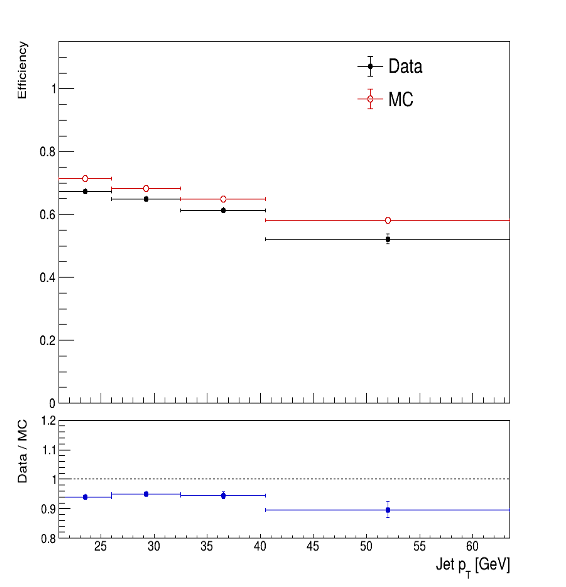
\includegraphics[width=0.48\linewidth]{Figures/mbd_vertex_efficiency/mbd_eff_mc_data_var_vs_jetpt.png}
    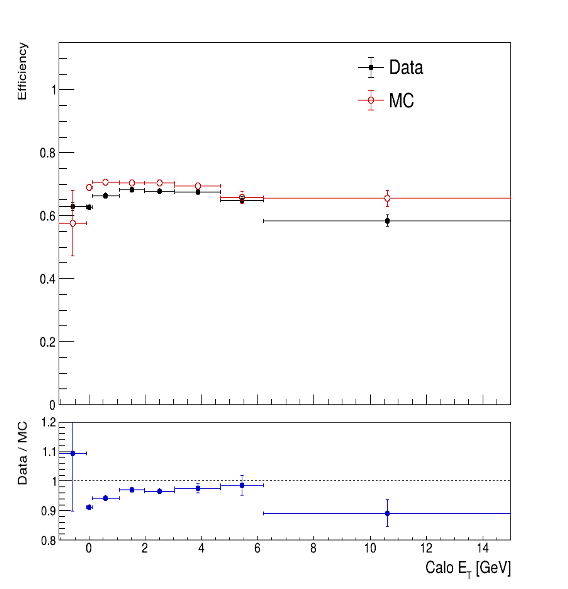
\includegraphics[width=0.48\linewidth]{Figures/mbd_vertex_efficiency/mbd_eff_mc_data_var_vs_et.png}
    \caption{MBD vertex efficiency as a function of leading jet $\pT$ (left) and transverse region $\Sigma E_{T}$ (right) for data and simulation.}
    \label{fig:mbd_vertex_efficiency_data_mc}
\end{figure}

\subsection{Unfolding Systematic Uncertainties}

\subsubsection{Prior reweighting}
The prior reweighting systematic uncertainty is derived by toggling on and off the reweighting of the prior distribution in the unfolding procedure.
Details of this reweighting procedure can be found in the unfolding section of the analysis note.
The overall effect of this prior reweighting on the UE measurement is found to be at the 2\% level for all leading jet $p_T$ bins.

\subsubsection{Herwig response}
The Herwig response systematic uncertainty is derived by using a response matrix derived from Herwig rather than Pythia to unfold the data and taking the difference as a systematic uncertainty on the UE measurement.
\textcolor{red}{The Herwig response systematic uncertainty is still being evaluated and will be added to the analysis note when it is finalized.}

\subsection{Total Systematic Uncertainty}
The total systematic uncertainty is found by adding the individual systematic uncertainties in quadrature.
Figure~\ref{fig:total_systematic_uncertainty} shows the contributions to the total systematic uncertainty on the UE measurement as a function of leading jet $p_T$.
The largest sources of uncertainty are from the calorimeter hadronic response, the pileup correction and the topocluster noise threshold.
\begin{figure}
    \centering
    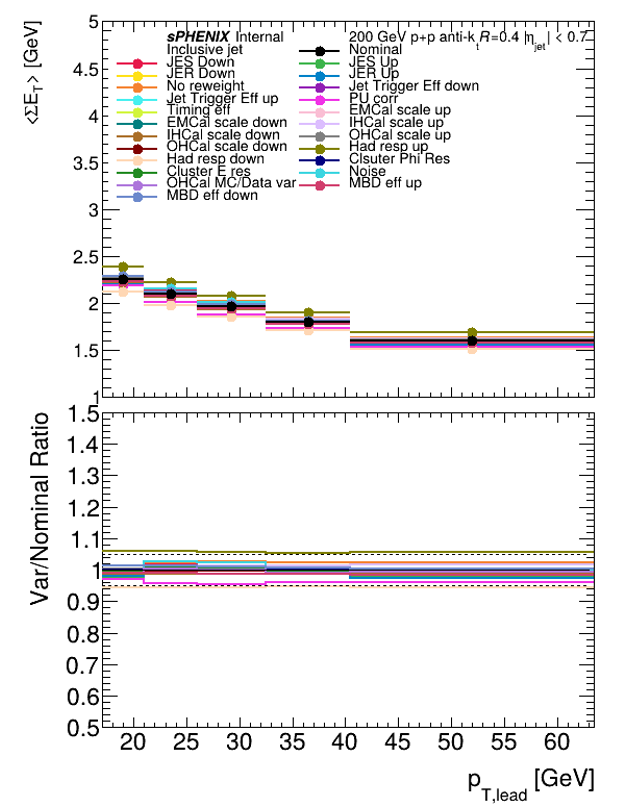
\includegraphics[width=0.48\linewidth]{Figures/systematics/h_syst_profile_inclusive.png}
    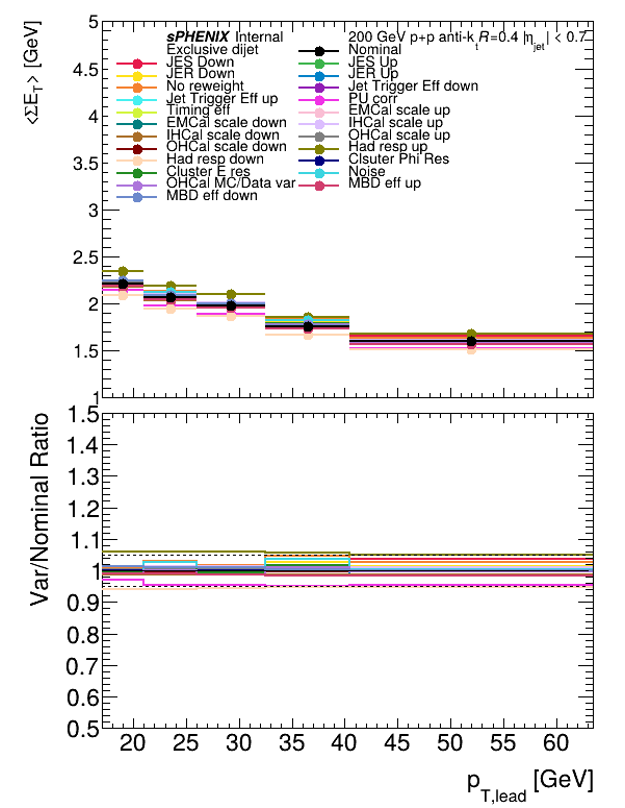
\includegraphics[width=0.48\linewidth]{Figures/systematics/h_syst_profile_dijet.png}
    \caption{Contributions to the total systematic uncertainty on the UE measurement as a function of leading jet $p_T$ for inclusive jet (left) and dijet (right) events.}
    \label{fig:total_systematic_uncertainty}
\end{figure}

The values of the systematic variations for the inclusive jet and dijet event results given in Figure \ref{fig:total_systematic_uncertainty} are shown in Table \ref{table:systematics}.
\begin{table}[ht]
\centering
\begin{tabular}{|c|c|c|}
\hline
Systematic Uncertainty & Inclusive Jet Variation & Dijet Variation \\ \hline
JES Down & 2.5\% & 3.62\% \\ \hline 
JES Up & -2.02\% & 1.75\% \\ \hline 
JER Down & -1.47\% & 2.82\% \\ \hline 
JER Up & -2.6\% & -1.43\% \\ \hline 
No reweight & 2.7\% & 4.6\% \\ \hline 
Jet Trigger Eff down & 0.00231\% & 0.00236\% \\ \hline 
Jet Trigger Eff up & 0.0036\% & 0.00446\% \\ \hline 
PU corr & -3.97\% & -4.48\% \\ \hline 
Timing eff & 0\% & 0\% \\ \hline 
EMCal scale up & 0.34\% & 0.368\% \\ \hline 
EMCal scale down & -0.224\% & -0.288\% \\ \hline 
IHCal scale up & 1.55\% & 1.43\% \\ \hline 
IHCal scale down & -1.32\% & -1.26\% \\ \hline 
OHCal scale up & 0.367\% & 0.41\% \\ \hline 
OHCal scale down & -0.245\% & -0.225\% \\ \hline 
Had resp up & 5.82\% & 6.08\% \\ \hline 
Had resp down & -5.57\% & -5.29\% \\ \hline 
Cluster Phi Res & 0.102\% & 0.129\% \\ \hline 
Cluster E res & 1.01\% & 1.64\% \\ \hline 
Noise & 2.53\% & 3.62\% \\ \hline 
OHCal MC/Data var & -0.709\% & 0.958\% \\ \hline 
MBD eff up & -1.7\% & -1.75\% \\ \hline 
MBD eff down & 1.25\% & 1.16\% \\ \hline 
\end{tabular}
\caption{Detailed values of systematic uncertainties for inclusive jet and dijet events.}
\end{table}
\label{table:systematics}
